\begin{frame}{Differential Power Analysis}
    \large{\centerline{\textbf{Introduction au side channel}}}

\end{frame}

\begin{frame}{CryptoBro en détresse \FiveStar \hfill 138 résolutions}
    \begin{columns}[c]
        \column{.45\textwidth}
        \begin{center}                  
            
\includegraphics[width=0.8\textwidth]{img/meme/cryptobros.png}
        \end{center}

        \column{.65\textwidth} % 
           \begin{outline}
               \1 Objectif
                \2 Récupérer le PIN d'un portefeuille crypto

            \pause
               \1 Données
                \2 Une trace courant pour chaque PIN
           \end{outline}
    \end{columns}
\end{frame}


\begin{frame}{Faillock et bypass}
    \centering
    \only<1>{
        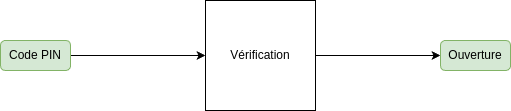
\includegraphics[width=0.6\textwidth]{img/sca/dfa/dfa-valid.drawio.png}
    }
    \only<2>{
        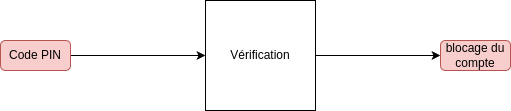
\includegraphics[width=0.6\textwidth]{img/sca/dfa/dfa-invalid.drawio.png}
    }
    \only<3->{
        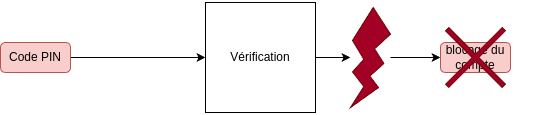
\includegraphics[width=0.6\textwidth]{img/sca/dfa/dfa-cutpower.drawio.png}
    }
\end{frame}

\begin{frame}{Comparaison séquentielle}
    \centering
    \only<1>{
        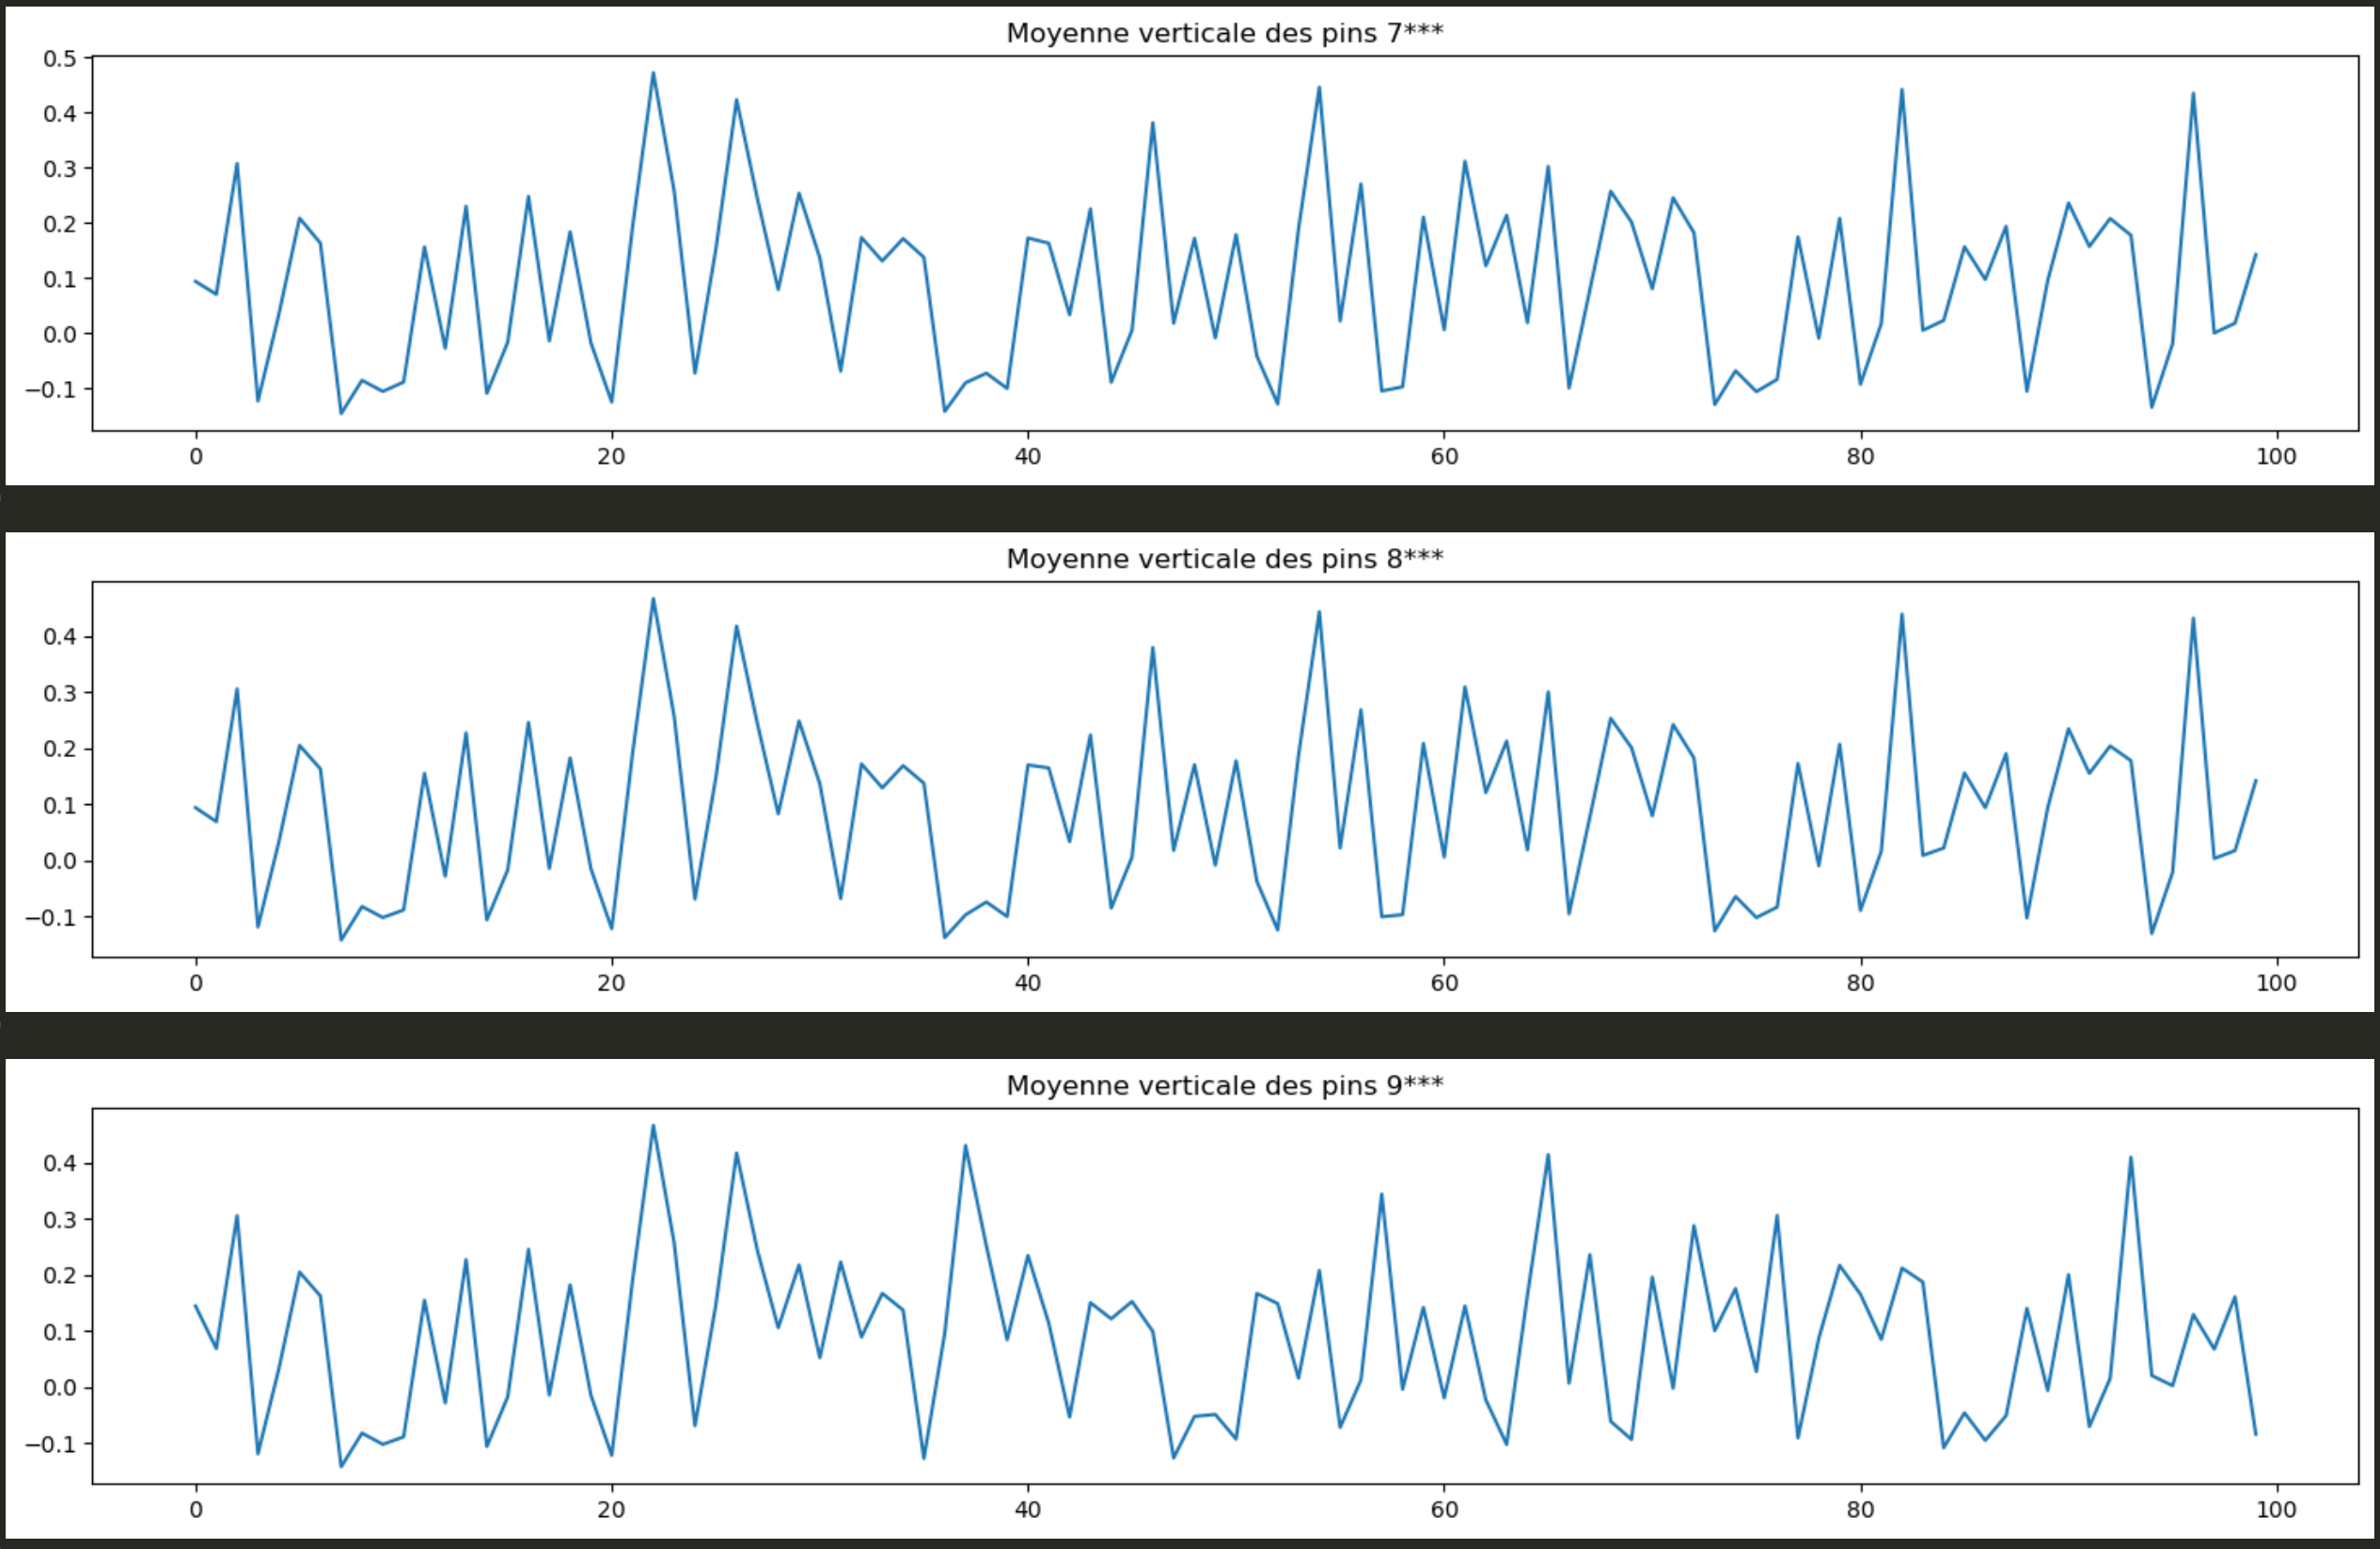
\includegraphics[width=0.7\textwidth]{img/sca/dfa/pin1.png}
    }
    \only<2>{
        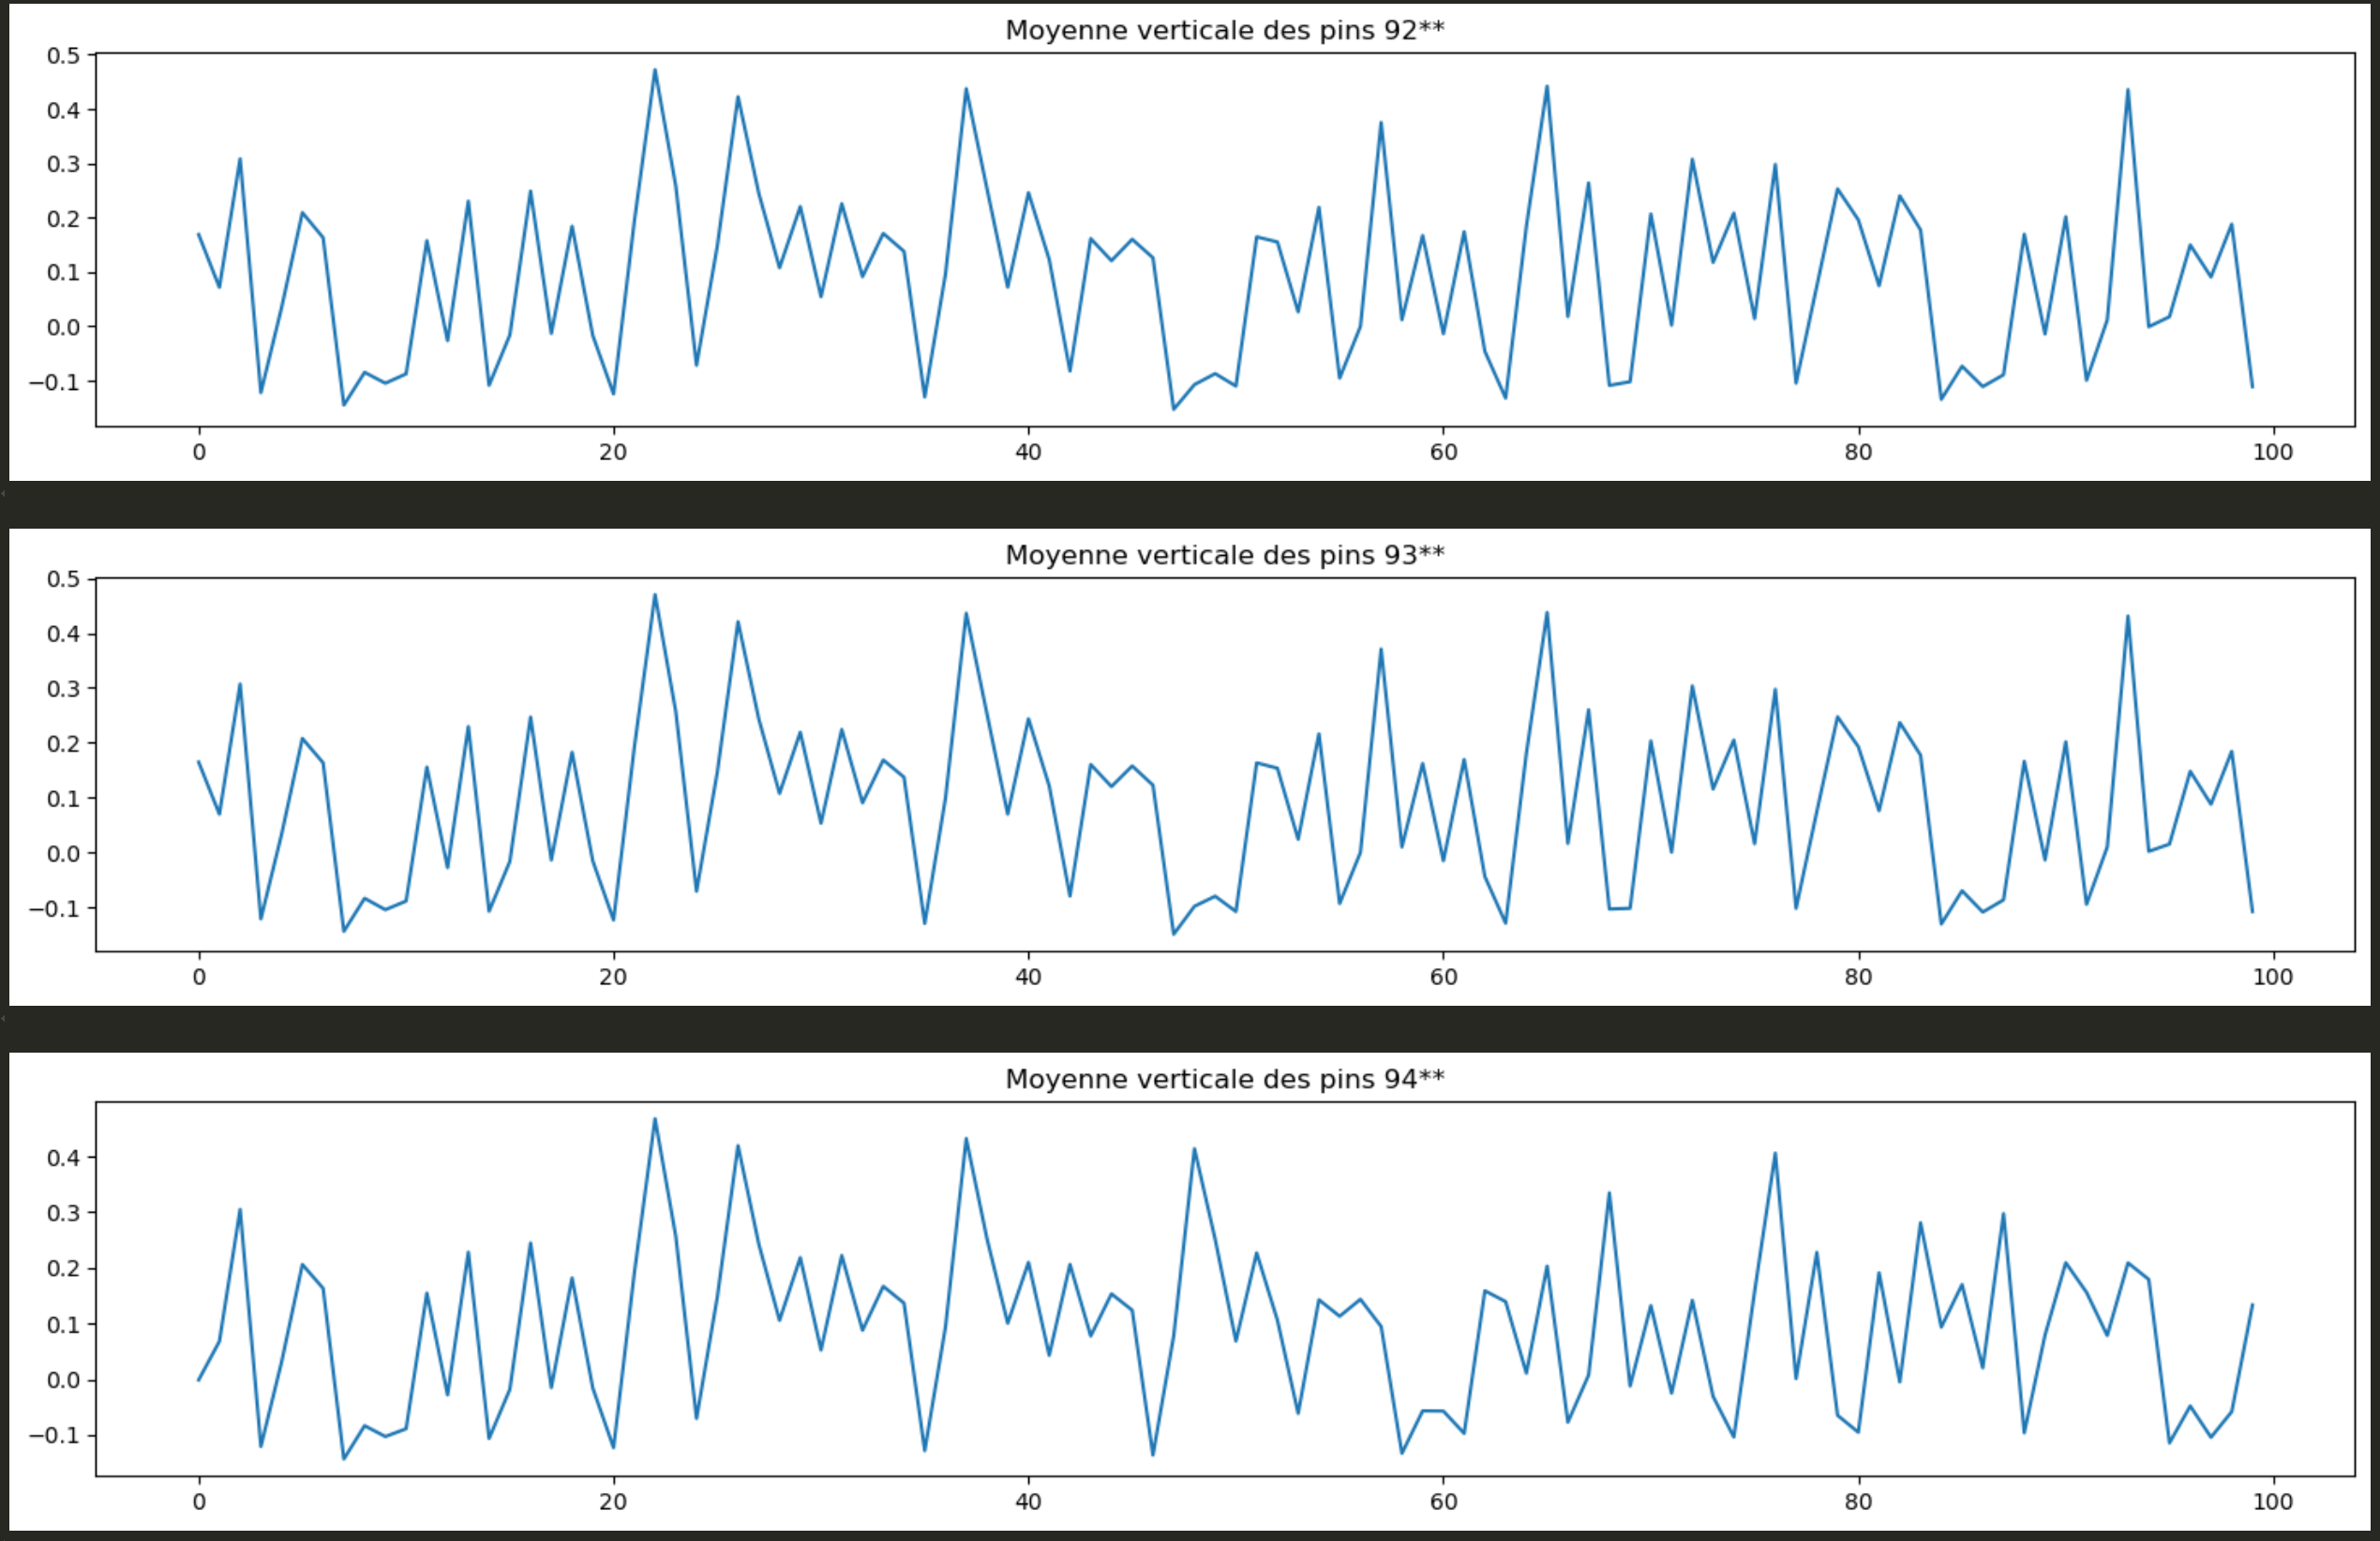
\includegraphics[width=0.7\textwidth]{img/sca/dfa/pin2.png}
    }
    \only<3>{
        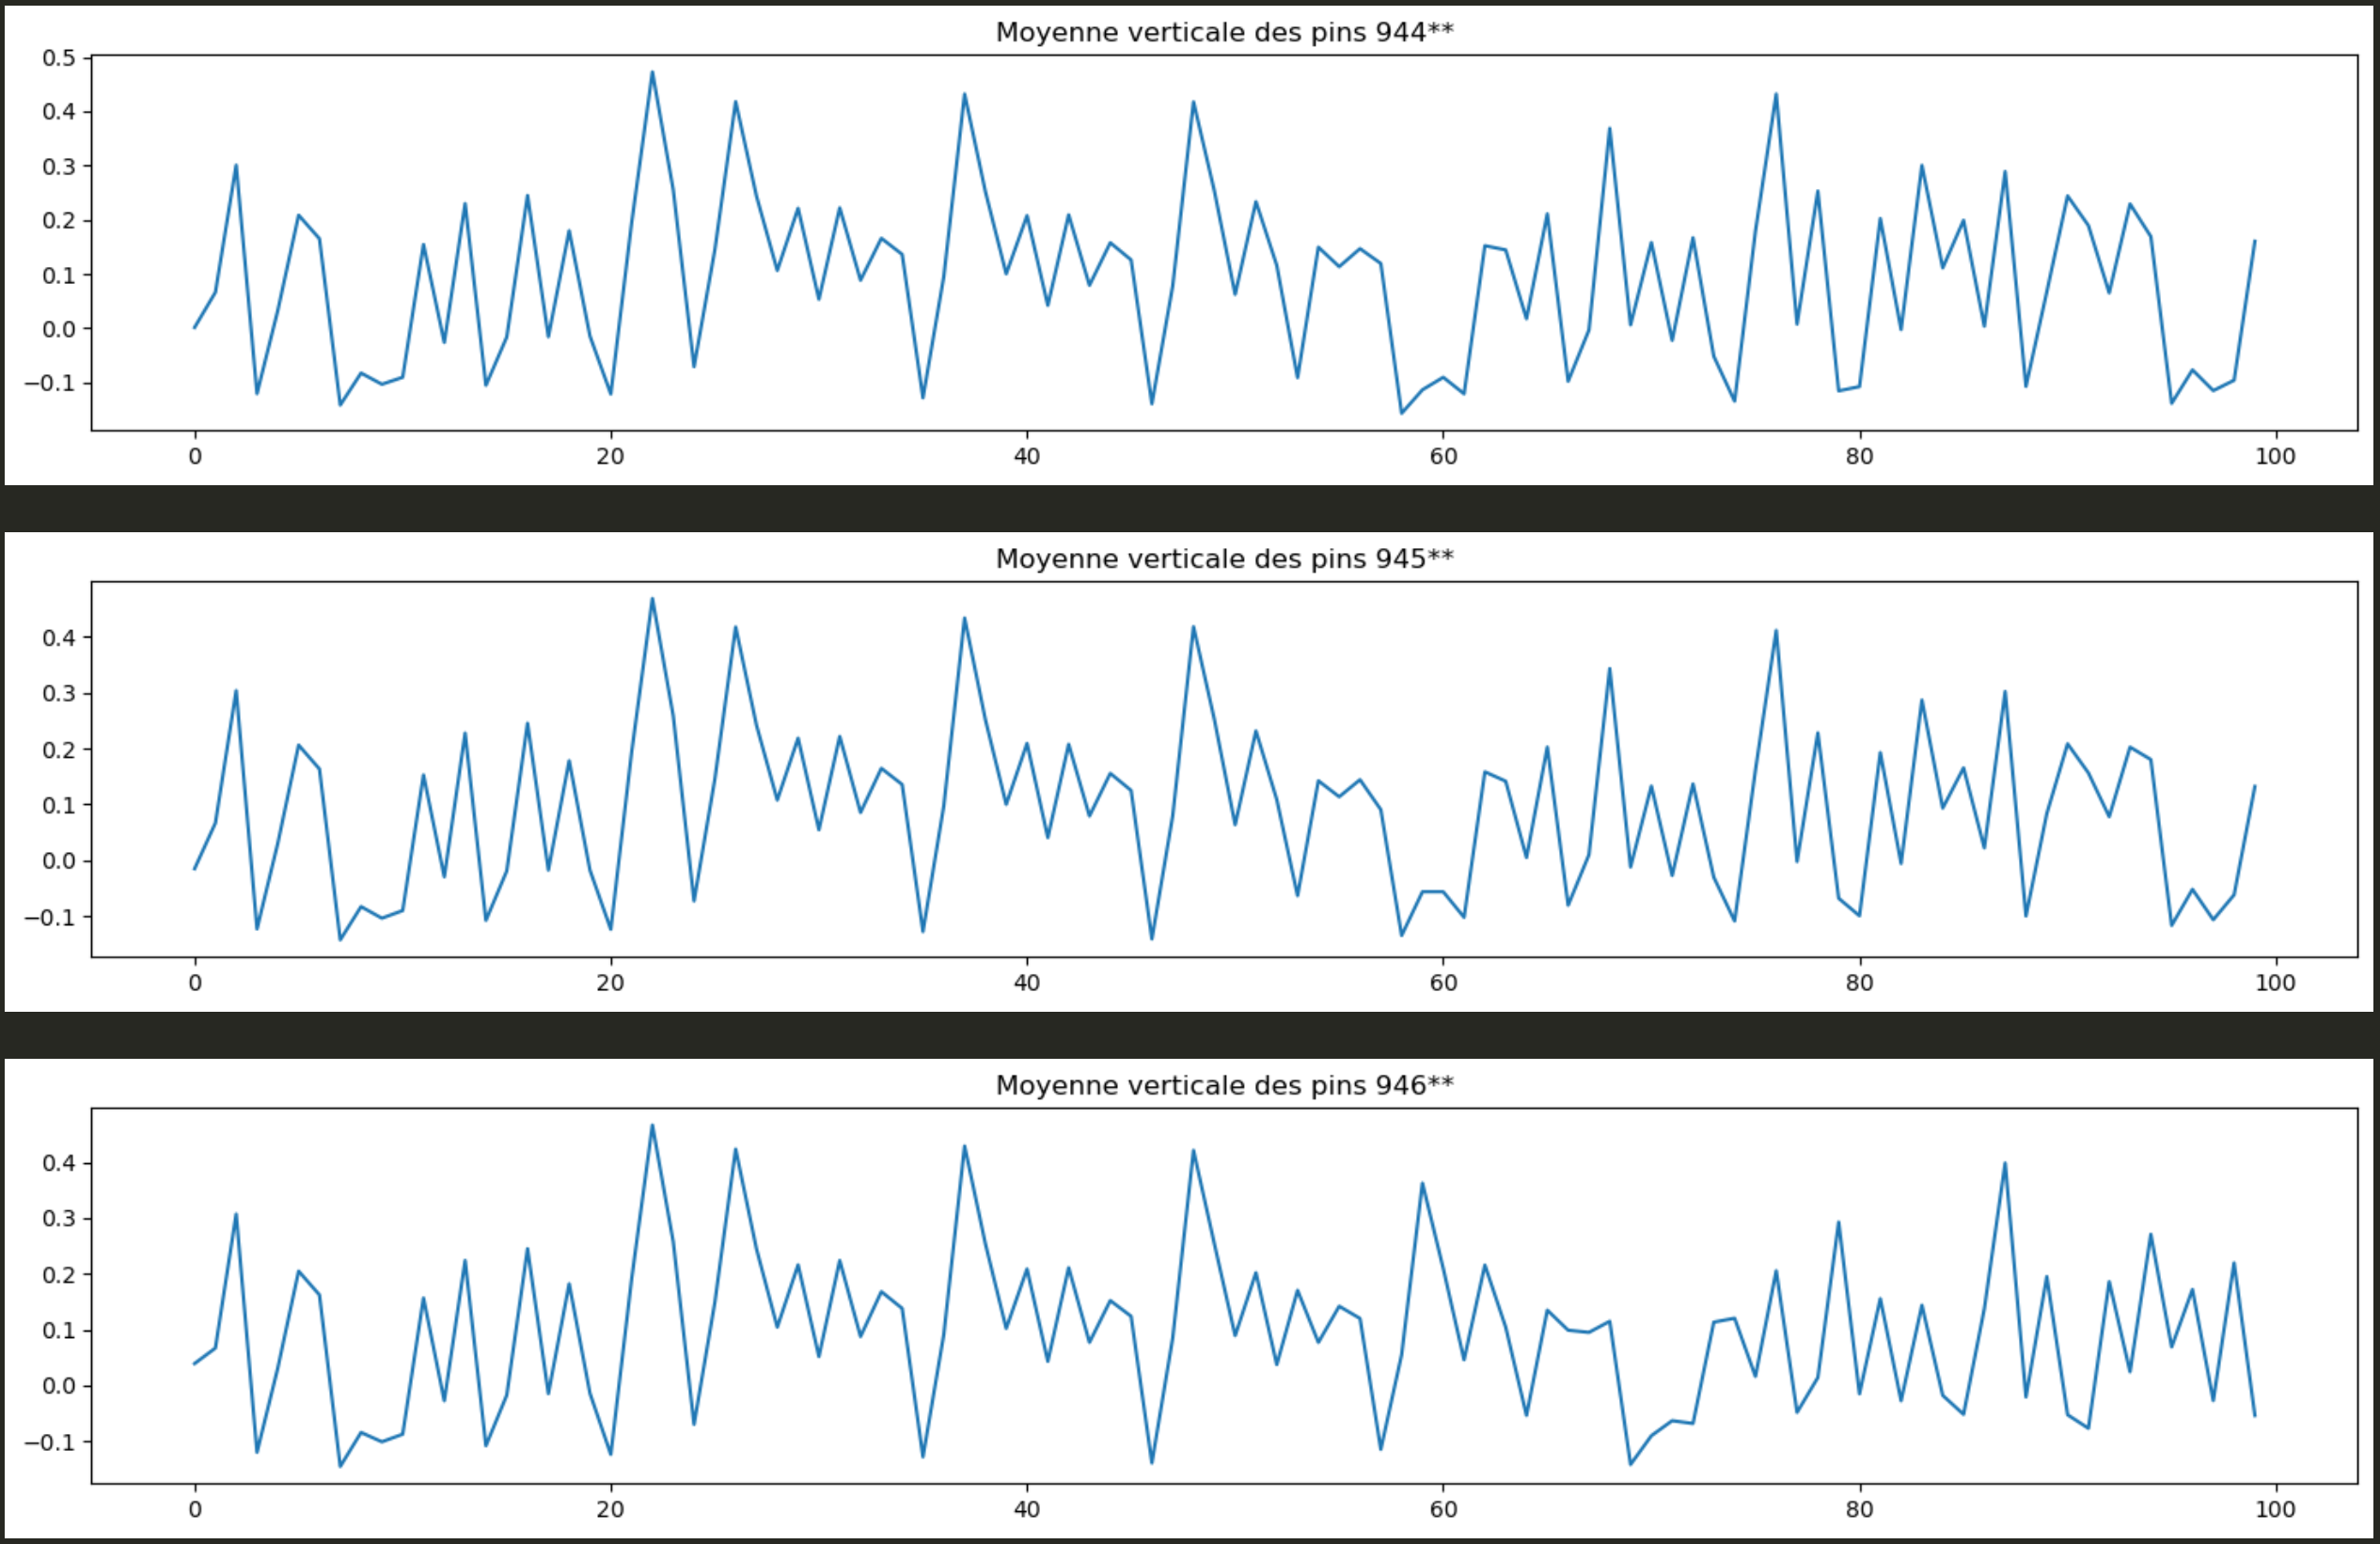
\includegraphics[width=0.7\textwidth]{img/sca/dfa/pin3.png}
    }
    \only<4->{
        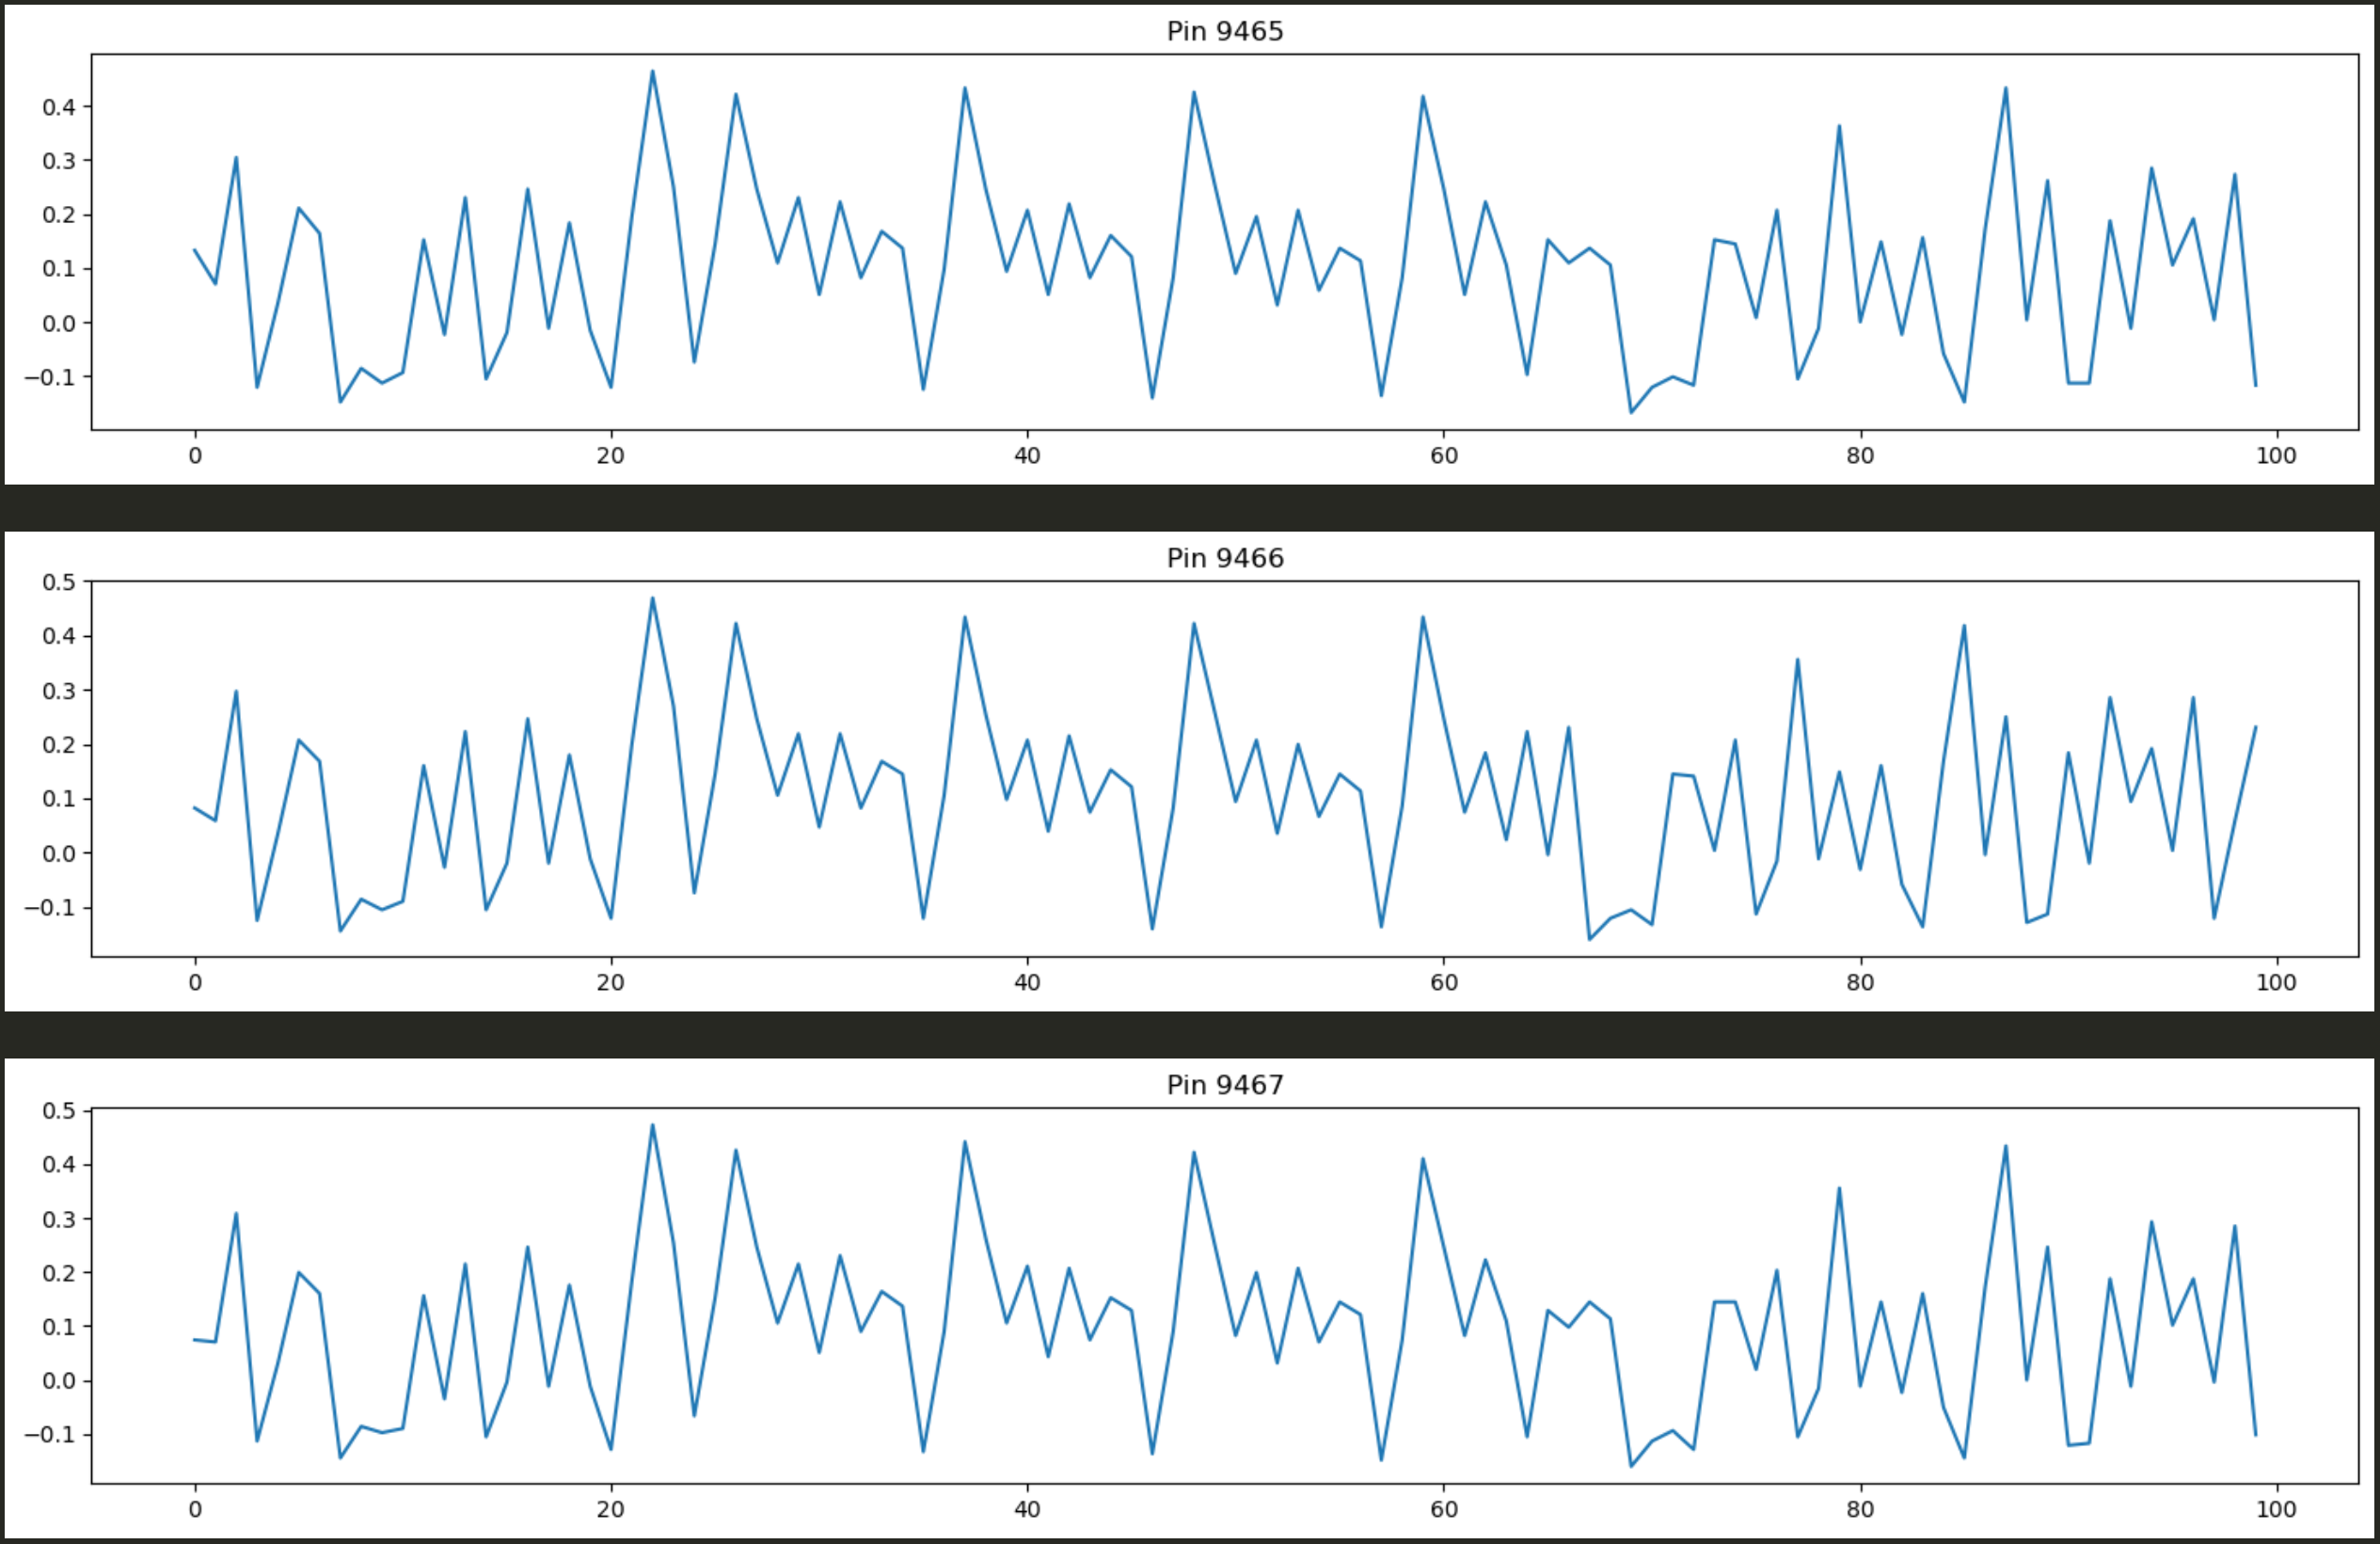
\includegraphics[width=0.7\textwidth]{img/sca/dfa/pin4.png}
    }
    \only<5>{\flag}
\end{frame}